\documentclass[12pt, twoside]{article}
\usepackage[letterpaper, margin=1in, headsep=0.2in]{geometry}
\setlength{\headheight}{0.6in}
%\usepackage[english]{babel}
\usepackage[utf8]{inputenc}
\usepackage{microtype}
\usepackage{amsmath}
\usepackage{amssymb}
%\usepackage{amsfonts}
\usepackage{siunitx} %units in math. eg 20\milli\meter
\usepackage{yhmath} % for arcs, overparenth command
\usepackage{tikz} %graphics
\usetikzlibrary{quotes, angles}
\usepackage{graphicx} %consider setting \graphicspath{{images/}}
\usepackage{parskip} %no paragraph indent
\usepackage{enumitem}
\usepackage{multicol}
\usepackage{venndiagram}

\usepackage{fancyhdr}
\pagestyle{fancy}
\fancyhf{}
\renewcommand{\headrulewidth}{0pt} % disable the underline of the header
\raggedbottom
\hfuzz=2mm %suppresses overfull box warnings

\usepackage{hyperref}

\fancyhead[LE]{\thepage}
\fancyhead[RO]{\thepage \\ Name: \hspace{4cm} \,\\}
\fancyhead[LO]{BECA / Dr. Huson / Geometry\\*  Unit 11: Circle angles, sectors, arcs \\* 2 March 2023}

\begin{document}

\subsubsection*{11.4 Homework: Mixed problems bank}
\begin{enumerate}
\item Find the volume of a pyramid ($V=\frac{1}{3}Bh$) having a height of 11.3 inches and with a square base having side lengths of 7 inches. Express your result to the \emph{nearest cubic inch}. %\vspace{5cm}

\item Find the volume of a hemisphere with a radius of 30 inches, to the \emph{nearest whole cubic inch}. (The formula for the volume of a \emph{sphere} is $V=\frac{4}{3}\pi r^3$) %\vspace{5cm}

\subsubsection*{Applying density ratios}
\item Find the weight of a metal block with a volume of 20 cubic inches and a density of 0.75 pounds per cubic inch. %\vspace{3cm}
\item A large block of ice has a volume of 45 liters. The density of ice (water) is one kilogram per liter. Find the weight of the ice.  %\vspace{3cm}
\item A tank of gasoline holds 20 gallons. Find the cost to completely fill the tank if gasoline costs \$2.35 per gallon. %\vspace{3cm}
\item A bar of solid gold is in the shape of a rectangular prism having a length of 10 cm, width of 4 cm, and thickness of 1.5 cm. The density of gold is 19.3 grams per cubic cm, and its approximate market value is \$50 per gram.
\begin{enumerate}
  \item Find the weight of the bar of gold.  %\vspace{3cm}
  \item Find its value in dollars.
\end{enumerate}

\item A tank of gasoline holds 15 gallons. Find the cost to completely fill the tank if gasoline costs \$3.15 per gallon. %\vspace{3cm}
\item A stick of butter has a volume of 90 cubic centimeters. If the density of butter is 0.9 grams per cubic centimeter, find the weight of a stick of butter. \vspace{3cm}
\item A large glass marble has a diameter of 3 cm. The density of glass is 2.70 $\mathrm{g/cm}^3$. Find the weight of the marble. %\vspace{3cm}

\item A bar of solid gold is in the shape of a rectangular prism having a length of 12 cm, width of 2 cm, and thickness of 2 cm. The density of gold is 19.3 grams per cubic cm, and its approximate market value is \$50 per gram.
\begin{enumerate}
  \item Find the weight of the bar of gold.  %\vspace{3cm}
  \item Find its value in dollars.
\end{enumerate}

\item A cylinder is 12.3 cm tall and has a volume of 966 cubic cm. Find the area of the base of the cylinder. Express your result to the \emph{nearest hundredth of a square centimeter}. %\vspace{3cm}

\item Find the volume of a pyramid ($V=\frac{1}{3}Bh$) having a height of 11.3 inches and with a square base having side lengths of 7 inches. Express your result to the \emph{nearest cubic inch}. %\vspace{5cm}

\item Find the volume of a hemisphere with a radius of 30 inches, to the \emph{nearest whole cubic inch}. (The formula for the volume of a \emph{sphere} is $V=\frac{4}{3}\pi r^3$)  %\vspace{5cm}

\item Given $R(-2,0)$ and $S(3,5)$, find the length of $\overline{RS}$. Simplify the radical.
\item Find the volume of a cone ($V=\frac{1}{3}\pi r^2 h$) having a height of 12 inches and with a radius of 3 inches. Express your result to the \emph{nearest cubic inch}. %\vspace{5cm}

\item Find the volume of a cylinder 10 inches tall with a radius of 6 inches, to the \emph{nearest whole cubic inch}. (The formula for the volume of a \emph{cylinder} is $V=\frac{4}{3}\pi r^3$)  %\vspace{5cm}

\subsubsection*{Model the situation with an equation. Use the formula sheet. You must start with a labeling variable. \hfill Do NOT solve!}

\item A large concrete post in the shape of a cylinder has a volume of 250 cubic feet. Its height is 12 feet. Find the radius of the base of the post. %\vspace{2cm}

\item A spherical cork fishing net float has a volume of 4000 cubic centimeters. Find its radius. %\vspace{2cm}

\item The volume of a cone having a \textbf{diameter} of 10 inches is 200 cubic inches. Find the cone's height. %\vspace{2cm}

\item A spherical cork fishing net float has a volume of 1700 cubic centimeters. Find its radius. %\vspace{2cm}

\item A large concrete post in the shape of a cylinder has a volume of 190 cubic feet. Its height is 11 feet. Find the radius of the base of the post. %\vspace{2cm}

\item The volume of a cone having a \textbf{diameter} of 9 inches is 48 cubic inches. Find the cone's height. %\vspace{2cm}


\subsubsection*{Applying density ratios}
\item A tank of gasoline holds 17 gallons. Find the cost to completely fill the tank if gasoline costs \$4.35 per gallon. \vspace{3cm}
\item A tub of lard has a volume of 100 cubic centimeters. If the density of lard is 0.85 grams per cubic centimeter, find the weight of the tub of lard. %\vspace{3cm}
\item A large glass marble has a diameter of 2.8 cm. The density of glass is 3.10 $\mathrm{g/cm}^3$. Find the weight of the marble. %\vspace{3cm}

\item A bar of solid gold is in the shape of a rectangular prism having a length of 18 cm, width of 8 cm, and thickness of 2.25 cm. The density of gold is 19.3 grams per cubic cm, and its approximate market value is \$55 per gram.
\begin{enumerate}
  \item Find the weight of the bar of gold.  %\vspace{3cm}
  \item Find its value in dollars.
\end{enumerate}



\newpage
\subsubsection*{Number line}
\item Given $\overleftrightarrow{RS}$ as shown on the number line, with $R=-3.1$ and $S=3.9$. \\[20pt] % Midpoint
  \begin{tikzpicture}
    \draw [<->] (-4.5,0)--(6.5,0);
    \foreach \x in {-4,...,6} %2 leading for diff!=1
      \draw[shift={(\x,0)},color=black] (0pt,-3pt) -- (0pt,3pt) node[below=5pt]  {$\x$};
      \draw [fill] (-3.1,0) circle [radius=0.05] node[above] {$R$};
      \draw [fill] (3.9,0) circle [radius=0.05] node[above] {$S$};
  \end{tikzpicture}
  \begin{enumerate}
    \item What is the exact distance on the number line between the points $R$ and $S$? \vspace{2cm} 
    \item The point $T$ bisects $\overline{RS}$. Find the value of $T$, and mark and label it on the numberline $\overleftrightarrow{RS}$ shown above. 
  \end{enumerate} %\vspace{2cm} 

\item In the diagram below, $\overline{AC}$ has endpoints with coordinates $A(-6,-3)$ and $C(6, 3)$.
\begin{center} %4 quadrant regents grid
  \begin{tikzpicture}[scale=.48]
    \draw [help lines] (-9,-5) grid (9,7);
    \draw [thick, <->] (-9.4,0) -- (9.4,0) node [below right] {$x$};
    \draw [thick, <->] (0,-5.4)--(0,7.4) node [left] {$y$};
    \draw [thick] (-6,-3)--(6, 3);
    \draw [fill] (-6,-3) circle [radius=0.1] node[above left] {$A$};
    \draw [fill] (6, 3) circle [radius=0.1] node[below right] {$C$};
  \end{tikzpicture}
\end{center}
If $B$ is a point on $\overline{AC}$ and $AB {:} BC = 1{:}3$,  what  are  the coordinates of $B$? %\vspace{5cm}

\item On the graph below, draw $\overline{AB}$, with $A(5,3)$ and $B(-1,-3)$, labeling the end points. Determine and state the coordinates of the midpoint $M$ of $\overline{AB}$ and mark and label it on the graph.\\
  \begin{tikzpicture}[scale=.635]
    \draw [help lines] (-3,-2) grid (8,7);
    \draw [thick, ->] (-3.2,0) -- (8.4,0) node [below right] {$x$};
    \draw [thick, ->] (0,-2.2)--(0,7.4) node [left] {$y$};
  \end{tikzpicture}
  \vspace{0.5cm}

\item Given $\overline{ABC}$, $AC=18$, and the point $B$ partitions $\overline{AC}$ in a ratio of 2:7.\\[0.5cm] Find ${AB}$. \\[1.5cm]
    \begin{tikzpicture}
      \draw [-, thick] (1,0)--(7,0);
      \draw [fill] (1,0) circle [radius=0.05] node[below]{$A$};
      \draw [fill] (3.5,0) circle [radius=0.05] node[below]{$B$};
      \draw [fill] (7,0) circle [radius=0.05] node[below]{$C$};
    \end{tikzpicture} %\vspace{3cm}

\newpage
\subsubsection*{Composition circle area and perimeter}
\emph{Unless otherwise instructed, find an exact answer, in terms of $\pi$ or using radicals if necessary.}

\item Use the formulas for the area and circumference of circles:
\[A=\pi r^2\]
\[C=\pi D = 2\pi r\]

\item Given the circle centered at $O$ with radius $r=3$. Leave an exact answer, in terms of $\pi$ if necessary.
\begin{multicols}{2}
  \begin{enumerate}
    \item Find the circumference of circle $O$. %\vspace{1cm}
    \item Find the area of the circle.\vspace{2cm}
  \end{enumerate}
  %\columnbreak
  \begin{tikzpicture}[scale=.635]
    \draw [help lines] (-5,-4) grid (5,4);
    %\draw [thick, ->] (-2.2,0) -- (10.4,0) node [below right] {$x$};
    %\draw [thick, ->] (0,-2.2)--(0,10.4) node [left] {$y$};
    \draw (0,0) circle [radius=3] node[below]{$O$};
    \draw [fill] (0,0) circle [radius=0.05];
  \end{tikzpicture}
\end{multicols}

  \item Find the radius of a circle having an area of $25 \pi$. \vspace{2cm}
  
  \item Find the area of the shape shown below composed of a rectangle and circular cap. Leave your answer as an exact value in terms of $\pi$.
    \begin{flushright}
    \begin{tikzpicture}[scale=.635]
      \draw [help lines] (-2,-1) grid (8,7);
      \draw [thick, ->] (-2.2,0) -- (8.4,0) node [below right] {$x$};
      \draw [thick, ->] (0,-1.2)--(0,7.4) node [left] {$y$};
      \draw [thick] (1,1)--(7,1)--(7,3)--(1,3)--cycle;
      %\draw [thick] (3,4) arc (90:270:1);
      \draw [thick] (7,3) arc (0:180:3);
    \end{tikzpicture}
  \end{flushright}\vspace{1cm}


\item Given the circle $C$ with circumference $10\pi$.
   \begin{enumerate}
     \item Write down the formula for the circumference of a circle and solve for the radius yielding a circumference of $6\pi$. \vspace{1cm}
     \item Find the area of the circle.
   \end{enumerate}
   \begin{tikzpicture}[scale=.635]
     \draw [help lines] (-4,-4) grid (4,4);
     %\draw [thick, ->] (-2.2,0) -- (10.4,0) node [below right] {$x$};
     %\draw [thick, ->] (0,-2.2)--(0,10.4) node [left] {$y$};
     \draw (0,0) circle [radius=3] node[below]{$C$};
     \draw [fill] (0,0) circle [radius=0.05];
   \end{tikzpicture}

\item Find the area of the shape shown below composed of a rectangle and a semi-circle.
  \begin{flushright}
  \begin{tikzpicture}[scale=.635]
    \draw [help lines] (-2,-1) grid (10,7);
    \draw [thick, ->] (-2.2,0) -- (10.4,0) node [below right] {$x$};
    \draw [thick, ->] (0,-1.2)--(0,7.4) node [left] {$y$};
    \draw [thick] (1,1)--(6,1)--(6,5)--(1,5)--cycle;
    \draw [thick] (6,1) arc (-90:90:2);
  \end{tikzpicture}
\end{flushright}


\item Given the circle $O$ with circumference $8\pi$.
  \begin{enumerate}
    \item Write down the formula for the circumference of a circle and solve for the radius yielding a circumference of $8\pi$. \vspace{1cm}
    \item Find the area of the circle.
  \end{enumerate}
  \begin{tikzpicture}[scale=.635]
    \draw [help lines] (-5,-5) grid (5,5);
    %\draw [thick, ->] (-2.2,0) -- (10.4,0) node [below right] {$x$};
    %\draw [thick, ->] (0,-2.2)--(0,10.4) node [left] {$y$};
    \draw (0,0) circle [radius=4] node[below]{$O$};
    \draw [fill] (0,0) circle [radius=0.05];
  \end{tikzpicture}

\item Use the formulas for the area and circumference of circles:
\[A=\pi r^2\]
\[C=\pi D = 2\pi r\]

\item Given the circle centered at $O$ with radius $r=4$. Leave an exact answer, in terms of $\pi$ if necessary.
\begin{multicols}{2}
  \begin{enumerate}
    \item Find the circumference of circle $O$. %\vspace{1cm}
    \item Find the area of the circle.\vspace{2cm}
  \end{enumerate}
  %\columnbreak
  \begin{tikzpicture}[scale=.635]
    \draw [help lines] (-5,-4) grid (5,4);
    %\draw [thick, ->] (-2.2,0) -- (10.4,0) node [below right] {$x$};
    %\draw [thick, ->] (0,-2.2)--(0,10.4) node [left] {$y$};
    \draw (0,0) circle [radius=4] node[below]{$O$};
    \draw [fill] (0,0) circle [radius=0.05];
  \end{tikzpicture}
  \end{multicols}

\item Find the radius of a circle having an area of $49 \pi$. \vspace{2cm}

\item Find the area of the shape shown below composed of a rectangle and circular cap. Leave your answer as an exact value in terms of $\pi$.
  \begin{flushright}
  \begin{tikzpicture}[scale=.635]
    \draw [help lines] (-2,-1) grid (8,7);
    \draw [thick, ->] (-2.2,0) -- (8.4,0) node [below right] {$x$};
    \draw [thick, ->] (0,-1.2)--(0,7.4) node [left] {$y$};
    \draw [thick] (2,1)--(6,1)--(6,3)--(2,3)--cycle;
    %\draw [thick] (3,4) arc (90:270:1);
    \draw [thick] (6,3) arc (0:180:2);
  \end{tikzpicture}
\end{flushright}\vspace{1cm}


\item Given $R(-1,1)$ and $S(3,4)$, find the length of $\overline{RS}$. Note: $l=\sqrt{(x_2-x_1)^2+(y_2-y_1)^2}$. %\vspace{4cm}

\item Given $R(-2,0)$ and $S(3,5)$, find the length of $\overline{RS}$. Simplify the radical. %\vspace{4cm}

\item Given $R(-3,1)$ and $S(5,7)$, find the length of $\overline{RS}$. Note: $l=\sqrt{(x_2-x_1)^2+(y_2-y_1)^2}$. %\vspace{4cm}

\item Given $P(7,0)$ and $Q(3,2)$, find the length of $\overline{PQ}$. Simplify the radical.


\item On the graph, draw polygon ABCDEF with vertices A(1, 1), B(1, 4), C(3, 4), D(3, 7), E(8, 7), and F(8, 1). Find the perimeter and the area of the polygon.\\[1cm]
\begin{tikzpicture}[scale=.635]
  \draw [help lines] (-2,-2) grid (10,10);
  \draw [thick, ->] (-2.2,0) -- (10.4,0) node [below right] {$x$};
  \draw [thick, ->] (0,-2.2)--(0,10.4) node [left] {$y$};
\end{tikzpicture}
\vspace{2cm}



\newpage
\subsubsection*{Estimating and measuring}
\item The point $P$ falls $A(0)$ and $B(10)$ on the numberline $\overleftrightarrow{AB}$ as shown below. \\[15pt] % Midpoint
\begin{tikzpicture}
  \draw [<->] (-0.5,0)--(10.5,0);
  \foreach \x in {0,10} %2 leading for diff!=1
    \draw[shift={(\x,0)},color=black] (0pt,-3pt) -- (0pt,3pt) node[below=5pt]  {$\x$};
    \draw [fill] (0,0) circle [radius=0.05] node[above] {$A$};
    \draw [fill] (10,0) circle [radius=0.05] node[above] {$B$};
    \draw [fill] (2*3.1416,0) circle [radius=0.05] node[above] {$P$};
\end{tikzpicture}
\begin{enumerate}
  \item Estimate the value of $P$ without using any tools. \vspace{1cm} 
  \item Find the position of $P$ as accurately as you can with a ruler. 
\end{enumerate} \vspace{1cm} 

\item The distance from $B$ on the line is scaled so that each centimeter represents one foot. \\[15pt] % Midpoint
\begin{tikzpicture}
  \draw [-] (0,0)--(10,0);
  \foreach \x in {0,...,10} %2 leading for diff!=1
    \draw[shift={(\x,0)},color=black] (0pt,-3pt) -- (0pt,3pt) node[below=5pt]  {$\x$};
    \draw [fill] (0,0) circle [radius=0.05] node[above] {$B$};
    \draw [fill] (3.5,0) circle [radius=0.05] node[above] {$M$};
    \draw [fill] (8.75,0) circle [radius=0.05] node[above] {$N$};
\end{tikzpicture}
\begin{enumerate}
  \item Estimate the distance of $M$ from $B$ in feet and inches (by eye). \vspace{1cm} 
  \item Using a ruler, find the distance between $M$ and $N$ in feet and inches. 
\end{enumerate} \vspace{2cm}

\item Given the circle $O$ with diameter $D=4$.
\begin{multicols}{2}
  \begin{enumerate}[itemsep=1.5cm]
    \item Estimate the area by counting the squares in the grid.
    \item Calculate the area. 
    \item Quantify the error in your estimate as a percentage.
  \end{enumerate}
  \begin{tikzpicture}[scale=1]
    \draw [help lines] (-3,-3) grid (3,3);
    %\draw [thick, ->] (-2.2,0) -- (10.4,0) node [below right] {$x$};
    %\draw [thick, ->] (0,-2.2)--(0,10.4) node [left] {$y$};
    \draw (0,0) circle [radius=2] node[below]{$O$};
    \draw [fill] (0,0) circle [radius=0.05];
  \end{tikzpicture}
\end{multicols}

\newpage
\item The diagram below is drawn to scale. Given that $BE=10$ and $DE=5$, find $AC$.
\begin{center}
  \begin{tikzpicture}[scale=1]
    \coordinate [label=left:$A$](A) at (-12,6);
    \coordinate [label=below:$B$](B) at (0, 0);
    \coordinate [label=below left:$C$](C) at (-12,0);
    \coordinate [label=above:$D$](D) at (-8, 4);
    \coordinate [label=below:$E$](E) at (-8,0);
    \draw [thick] (A)--(B)--(C)--cycle;
    \draw [thick] (A)--(C);
    \draw [thick] (D)--(E);
  \end{tikzpicture}
\end{center}

\item In right triangle $ABC$ shown below, point $D$ is on $\overline{AB}$ and point $E$ is on $\overline{BC}$ such that $\overline{AC} \parallel \overline{DE}$. Given $BD=10$, $BC=12$, and $EC=4$.
  \begin{center}
    \begin{tikzpicture}[scale=0.7]
      \coordinate [label=left:$A$](A) at (-12,6);
      \coordinate [label=below:$B$](B) at (0, 0);
      \coordinate [label=below left:$C$](C) at (-12,0);
      \coordinate [label=above:$D$](D) at (-8, 4);
      \coordinate [label=below:$E$](E) at (-8,0);
      \draw [thick] (A)--(B)--(C)--cycle;
      \draw [thick] (A)--(C);
      \draw [thick] (D)--(E);
    \end{tikzpicture}
  \end{center}
\begin{enumerate}
  \item Find the length of $\overline{BE}$. \vspace{0.5cm}
  \item Find the scale factor, $k$, dilating $\triangle DBE \rightarrow \triangle ABC$, centered at $B$. \vspace{1.5cm}
  \item Find the area of $\triangle ABC$. %\vspace{2.5cm}
  \item Find the area of $\triangle DEB$. %\vspace{2.5cm}
  \item Find the ratio of the areas of the two triangles. %\vspace{2.5cm}
  \end{enumerate}

\newpage
\item Given $m\angle R=45$ and $m\angle UST=110$. Find $m\angle U$.\\[1cm]
  \begin{tikzpicture}
    %\draw [->, thick] (0,0)--(5,5);
    \draw [<-, thick] (8,0)--(0,0)--(3,3)--(4.5,0);
    \draw [fill] (0,0) circle [radius=0.05] node[below]{$R$};
    \draw [fill] (4.5,0) circle [radius=0.05] node[below]{$S$};
    \draw [fill] (3,3) circle [radius=0.05] node[right]{$U$};
    \draw [fill] (7,0) circle [radius=0.05] node[below]{$T$};
  \end{tikzpicture}
  %\vspace{2cm}

\item In  $\triangle ABC$ shown below, side $\overline{AC}$ is extended to point $D$ with $m\angle DAB=(6x-9)^\circ$, $m\angle C=35^\circ$, and $m\angle B=(4x+4)^\circ$.
  \begin{center}
    \begin{tikzpicture}
      \draw [thick](-1.5,0)node[below]{$D$}--
        (1.8,0)node[below]{$A$}--
        (9,0)node[below]{$C$}--
        (4,3)node[above]{$B$} --(2,0);
        \node at (2.2,0)[above left]{$(6x-9)^\circ$};
        \node at (8.2,0)[above left]{$35^\circ$};
        \node at (4.4,2.4)[below]{$(4x+4)^\circ$};
    \end{tikzpicture}
  \end{center}
  What is $m\angle BAC$?

  \item On the set of axes below, graph the quadrilateral $ABCD$ having coordinates $A(-3,-3)$, $B(5,1)$, $C(6,8)$, and $D(-2,4)$.
    \begin{center} %4 quadrant regents grid
    \begin{tikzpicture}[scale=.48]
      \draw [help lines] (-9,-9) grid (9,9);
      \draw [thick, <->] (-9.4,0) -- (9.4,0) node [below right] {$x$};
      \draw [thick, <->] (0,-9.4)--(0,9.4) node [left] {$y$};
      %\draw [thick] (-3,-3) node[below] {$A$}--
      %(5,1) node[right] {$B$}--
      %(6,8) node[left] {$C$}--
      %(-2,4) node[left] {$D$}--cycle;
      %\draw [fill] (5,0) circle [radius=0.1] node[above left] {$P$};
    \end{tikzpicture}
    \end{center}
    Show that the midpoints of the two diagonals, $\overline{AC}$ and $\overline{BD}$, are the same point. \\%[5cm]
    Prove $ABCD$ is a parallelogram. Use the following theorem:
    A quadrilateral is a parallelogram if and only if its diagonals bisect each other. \\[0.5cm]
    Be sure to state the conclusion in your proof.








  
\newpage
\item Perform each calculation, writing down the full calculator display and then rounding to the \emph{nearest hundredth}.
\begin{multicols}{2}
\begin{enumerate}
  \item $V=\frac{1}{3} \pi (2.4)^2(5.1)$
  \item $P=3.6 + \frac{1}{2} \pi (3.6)$  
\end{enumerate}
\end{multicols}\vspace{2cm}

\item Solve each equation for the appropriate variable. Do not round. Simplify radicals.
\begin{multicols}{2}
\begin{enumerate}[itemsep=2cm]
  \item $A=\pi r^2=27\pi$
  \item $V=\frac{1}{3}(6.0)^2h=153$  
\end{enumerate}
\end{multicols}%\vspace{5cm}

\item Perform each calculation, writing down the full calculator display and then rounding to the \emph{nearest hundredth}.
\begin{multicols}{2}
\begin{enumerate}
  \item $V=\frac{1}{3} \pi (2.7)^2(1.1)$
  \item $W=5.1 + \frac{1}{2} \pi (7.1)$  
\end{enumerate}
\end{multicols} %\vspace{2cm}

\item Solve each equation for the appropriate variable. Do not round. Simplify radicals.
\begin{multicols}{2}
\begin{enumerate}%[itemsep=2cm]
  \item $A=\pi r^2=18\pi$
  \item $V=\frac{1}{4}(2.2)^2h=12.1$
\end{enumerate}
\end{multicols}%\vspace{5cm}

\item Perform each calculation, writing down the full calculator display and then rounding to the \emph{nearest hundredth}.
  \begin{multicols}{2}
  \begin{enumerate}%[itemsep=4cm]
    \item $A=15.944732$
    \item $W=3.4 \times 9.8 \times 4.3 \times 0.15$
          
    \item $V=\frac{1}{3} \pi (3.4)^2(6.1)$
    \item $P=8.6 + \frac{1}{2} \pi (8.6)$  
    \item $V=199.19711$
    \item $W=\frac{1}{3} (13)  3.3^2 \times 1.175$
    \item $V=\frac{1}{3} \pi (12.4)^2(8.1)$
    \item $P=12 + \frac{1}{4} \pi (12)$ 
  \end{enumerate}
  \end{multicols}%\vspace{2cm}

\item Perform each calculation, writing down the full calculator display and then rounding to the \emph{nearest hundredth}.
  \begin{multicols}{2}
  \begin{enumerate}%[itemsep=4cm]
    \item $A=15.944732$
    \item $W=3.4 \times 9.8 \times 4.3 \times 0.15$
          
    \item $V=\frac{1}{3} \pi (3.4)^2(6.1)$
    \item $P=8.6 + \frac{1}{2} \pi (8.6)$  
    \item $V=199.19711$
    \item $W=\frac{1}{3} (13)  3.3^2 \times 1.175$
    \item $V=\frac{1}{3} \pi (12.4)^2(8.1)$
    \item $P=12 + \frac{1}{4} \pi (12)$ 
  \end{enumerate}
  \end{multicols}%\vspace{2cm}

\newpage
\item Express the result to the nearest thousandth.  \vspace{1cm}
  \begin{multicols}{2}
    \begin{enumerate}
      \item $\sin 35^\circ = $ \vspace{1cm}
      \item $\tan 70^\circ =$
      \item $\sin 78^\circ = $ \vspace{1cm}
      \item $\cos 12^\circ =$
    \end{enumerate}
  \end{multicols} \vspace{0.5cm}


\end{enumerate}
\end{document}